\documentclass[twoside,a4paper]{article}

\usepackage{graphicx}
\usepackage{url}
\usepackage{verbatim}
\usepackage{pgfplots}
\usepackage{tikz}
\usepackage{amsmath}
\usepackage{amsfonts}
\usetikzlibrary{arrows,shapes}
\usepackage{listings}
\title{ Building a multimodal co-occurence-based recommender engine with Apache Mahout and Apache Solr }
\author{
	Author \\
	Lukas Hofmaier \\
	lukas.hofmaier@hsr.ch
 	\and
	Supervisors \\
        Hansj''org Huser
}
\date{
	\textsc{University of Applied Sciences Rapperswil}\\
	Project Thesis,
	\today
}
\begin{document}
\maketitle
\tableofcontents

\begin{abstract}
The behavior of users provide data to predict the relevance of recommendations to individual users. The recommender engine discussed in this article has a two part design.
Co-occurence can be computed at scale with Apache Mahout's \verb|spark-itemsimilarity| job.
Recommendations are query results of the search engine Apache Solr.
\end{abstract}

\section{Introduction}
\label{sec:intro}

\subsection{Recommender engines}
\label{sec:recommenderengines}

Recommender engines are services that recommend articles (items) to users based on their past actions. They attempt to infer taste and preferences. A recommender engine presents the user previously unknown items that are of interest for the user. 

For example, if a user has purchased the movies "Terminator 2" and "Transformers" the recommender engine will present the activ user a list of other similar movies.

E-commerce sites that deploy a recommender engine can have a increase in sales of 8 - 13 percent \footnote{http://www.practicalecommerce.com/articles/1942-10-Questions-on-Product-Recommendations}.

\subsection{Strategies}
\label{sec:strategies}

There are different strategies to discover to recommend a user new items \cite{Owen}.
\begin{description}
\item[Collaborative Filtering] This strategy is only based on the preference or taste information from many users. For example, a recommender engine based on collaborativ filtering uses the ratings of all users to compute the similarity between all items. 

It requires no knowledge of the properties of the items. Recommender engines based on collaborative filtering do not care what the items are and what attributes they have. This can be an advantage because the same technique can be applied to different types of items. 

User preferences will change over time. Another advandage is that collaborative filtering will update the model automaticaly as it's exposed to new user histories. The systems learns.
\item[Content based filterting] Content-based recommendation techniques use attributes of the items in order to predict preferences of users. For example, if a recommender recommends movies of a Steven Spielberg because the active user likes other movies of Steven Spielberg it uses content based filtering.
\end{description}

This article describes a recommender engine based on collaborative filtering. The recommendations are only based on user input. The recommender engine is designed to mixe any number of user actions (clicks, purchases, likes, tags). The ratings of a user and the applied tags will be used to compute recommendations.

\subsection{Challenges and Problems}

There are serveral ways to design and build a recommender eninge \cite{Dunning14}.

\begin{itemize}
\item Design a custom recommender engine. That approach requires a team of highly trained engineer and data scientist.
\item Use products that offer drag-and-drop approaches. Some of these product try to automaticaly select the right algorithms. This recommender engines aren't very effective and a most of the effort required is put into getting the data into the right format.
\item Use the service of a high-end machine-learning consultancy. These companies achieve effective results by trying a huge collection of algorithms at each problem and selecting the algoritm that gives the best result.
\end{itemize}

There are several problem and challenges in building a recommender engine:
\begin{itemize}
\item Many algorithms relies on user ratings. Ratings come from a subset of users. Only user who like to rate will rate items. 
\end{itemize}

In this article we use a simplified approach to the recommender problem described in \cite{Dunning14}. The goal of the apporach presented in this article is to provide a simple solutions that gives the user practical recommendation. There are academic approaches that produce recommendation with a smaller error but these require complex mathematical models. The goal of the apporach presented in this article is to provide a simplified, general solution for the recommender problem. In contrast to an academic approach it is easiear to extend the recommender engine to a multimodel recommender.


Many existing collaborativ filtering type recommenders use one user activity to model preference \cite{ferrel}. But a variety of user activities can be use in combination to improve the quality of recommendations. Section \ref{sec:design} will describe how different type of interactions is used as input data to train the recommender.

The recommender described in this article is divided in two parts.
\begin{itemize}
\item Computation of simililarity and the update of the text search engine is done offline, ahead of time.
\item Recommendations are generated instantly by quering the text search eninge using rescents actions of the user.


\end{itemize}

\subsection{Overview}

Section \ref{sec:design} will describe the design of the co-occurence based recommender. The similiarity metric log-likelihood ratio is described and a short introduction for the search engine Apache Solr is given.


\section{Co-occurence based multimodal recommender}
\label{sec:design}
\tikzset{
  reco/.style={
    rectangle
  },
}

\begin{figure}
  \centering
  \begin{tikzpicture}[->, >=latex]
    \node[reco] (rec) at(180:3cm) {Recommender};
    \node (hist) at(60:3cm){History};
    \node (se) at(300:3cm){Search engine};
    \node (user) [left of=rec,node distance=5cm]{User};
    \node(x)[align=left] at(130:3.9cm){lookup\\ user's history};
    \node(x)[align=left] at(0:2cm){user's\\ history};
    \node(x)[align=left] at(220:4cm){ranked \\ search result};
    \draw[->, >=latex] (170:3cm) arc  (170:80:3cm);
    \draw[->, >=latex] (40:3cm)  arc (40:-40:3cm);
   \draw[->, >=latex] (270:3cm)  arc (270:190:3cm);
   \draw[->, >=latex] (40:3cm)  arc (40:-40:3cm);
   \path (user) edge[bend left=40] node[anchor=south,above]{request top-N list}(rec);
   \path (rec) edge[bend left=40] node[anchor=north,below]{top-N list}(user);
  \end{tikzpicture}
  \caption{Simplified dataflow diagram}
  \label{fig:topndataflow}
\end{figure}

The recommender we discuss will use past user behavior and metadata of items to compute the similarity between all items. Hence it is a hybrid recommender.
We use user \gls{coocc} of user- and tag-iteminteractions as a similarity metric among items.

Because search engine are a way of finding similar documents according to a query we can use a search engine to find similar items to the ones the user already exressed some interest.

The process of procucing a \gls{topn} can be divided into five steps. Figure \ref{fig:topndataflow} illustrates this process.

\begin{enumerate}
\item User requests a \gls{topn}.
\item The recommenders looks up items that appear in the recent user history.
\item The user's action history the recommender is send as a query to the search engine.
\item The search engine returns a ranked search result set of items according to the query.
\item The recommender removes item already known to the user and present him a \gls{topn}.
\end{enumerate}

The section first describes the used input data. Than we explain the process of computing \gls{topn} and how similarity between items is measured and how the computation is implemented. Next we describe the similarities of the top-N recommender task and a \gls{rankedretrieval} and how we extend the scoring function of the search engine in order to use \gls{coocc} similaty metric.

\subsection{Record user behavior}
\label{sec:inputdata}

\begin{figure}
  \centering
     \includegraphics[width=0.9\textwidth]{collectinginput}
  \caption{The user can like and tag movies with the web front end. The user actions are recorded by the web server.}
  \label{fig:gui}
\end{figure}

The \gls{rec} suggests items that are similar to the ones the user already liked in the past. In order to build a model for similarity we need to train the recommender with some data about the items.
This section will descibe the type of input data we use  in our demo application. The report will refer to this type of input data. 

Many collaborative filtering recommender engines use excplicit user ratings to train their model. Explicit user ratings of a user for an item are expressed by numbers (e.g. a rating is a number between 1 and 5). The use of explicit feedback has some drawbacks.
\begin{itemize}
\item Only a small subset of users will rate items. This leads to a model that is skewed against user who like to rate.
\item The majority of ratings are associated with a small fraction of the most popular items \cite{Anderson}. As a result it is less likely that unknown items show up in the \gls{topn}. This behavior is undesirable because the goal of the recommender is to present items the a user would not find on his own.
\end{itemize}

Corresponding to \cite{Dunning14} the best choice of input data is the collection past user actions on a website. The stored behavior of one user is called the user's \gls{history}. It shows what users actually do. Hence the input data should consist of recorded \glspl{useraction} (e.g. purchase, view, like, tag).

In our demo web application we record two different user actions:
\begin{description}
\item[like]  Users can express their positive feedback for a movie by clicking on a ``like'' button (the \gls{like} action is an explicit rating. We use it instead of a purchase or view action in order to keep the GUI simple).
\item[tag] User can \gls{tag} items. Every item can be associated with a list of \glspl{tag}.
\end{description}
The recorded like and tag action are later used to compute similarity between items.
Figure \ref{fig:gui} shows the simplistic user interface of our demo web app.

The web browser sends every user action to the web server. The web server provides a REST Web API that receives the \glspl{useraction} as HTTP \verb|Post| request and saves them to a sqlite3 \footnote{https://www.sqlite.org/} database.

In order to analyse the data later we want to retrieve the action history $h_u$ for a particular user $u$ for a defined action and a list of tags for every item. Hence we have to structure the data accordingly. Figure \ref{fig:er} shows the entity relationship diagram for the user actions \gls{like} and \gls{tag}

\tikzset{multi  attribute/.style={attribute ,double  distance=1.5pt}}
\tikzset{derived  attribute/.style={attribute ,dashed}}
\tikzset{total/.style={double  distance=1.5pt}}
\tikzset{every  entity/.style={draw=blue , fill=blue!20}}
\tikzset{every  attribute/.style={draw=yellow, fill=yellow!20, node distance=1.0cm}}
\tikzset{every  relationship/.style={draw=red, fill=red!20}}

\begin{figure}
\centering
\begin{tikzpicture}[node distance=2.0cm]
  \node[entity](user){user};
  \node[relationship](like)[above right of=user]{ like } edge (user);
  \node[attribute](date2)[above of=like]{ date } edge (like);
  \node[entity](item)[below right of=like]{item} edge (like);
  \node[relationship](tag)[below right of=user]{ tag } edge (user) edge (item);
  \node[attribute](text)[below right of=tag]{ text } edge (tag);
  \node[attribute](date1)[below left of=tag]{ date } edge (tag);
  \end{tikzpicture}
\caption{The data model allows us to retrieve the action history for every user. Like and tag form associations of user with item.}
\label{fig:er}
\end{figure}

It makes sense to start recording behavioral data month's before depoying the recommender engine because the recommender engine has to analyze the data and build a model of similarty among items in order to create personalized recommendations.


\subsection{How to compute the top-N recommendations list?}
\label{sec:problem}
This section gives a mathematical description of the top-N recommendation task and hence it describes the computations required to produce recommendations. The description refers to the \gls{rec}.

Suppose we have a metric to express similarity between two items as a numerical value and the magnitude of the value determines the strength of similarity. If we compute the similarity for every item pair in a set of $n$ items, we can represent the result in a matrix $M$. $M$ is a $n \times n$ matrix. Each row and each column contains the similarities between one particular item and all other items. $M$ is symetric across the diagonal because the similarity between $a$ and $b$ must be the same as between $b$ and $a$ (commutativity). The diagonal of $M$ contains the value for maximum similarity because this value represents the comparison of an item to itself. $M$ is called the \gls{indicatorm}. Equation \ref{eq:similaritymatrix} shows an example of an \gls{indicatorm} with 4 items.

\begin{equation}
  \label{eq:similaritymatrix}
M =\bordermatrix{~ & 1 & 2 & 3 & 4 \cr
 1 & 1  & 0.40 & 0.9 & 0.1 \cr
2 & 0.40 &1  & 0.9 & 0.1 \cr
 3& 0.9 & 0.9 &1  & 0.63 \cr
 4 & 0.1 & 0.1 & 0.63 &1  \cr}
\end{equation}
Further we represent a user action history for each user as vector $h_l$ of length $n$. $h_l$ contains an element for every item. The user's interactions with an item are represented as binary values in $h_l$. If the there is an interaction with an item in the history the value or the corresponding element is 1. Otherwise the value is 0. For example equation \ref{eq:history} shows a user's action history for the action ``like''. He has liked item 1 and 2.

\begin{equation}
\label{eq:history}
h_l =
\begin{pmatrix}
 1 \\
 1 \\
 0 \\
 0 \\
\end{pmatrix}
\end{equation}

To create a \gls{topn} for user $u$ we compute the matrix vector product of $M$ and $h_l$. The result $r$ is a vector of length $n$, that contains a value for every item. $r$ maps every item to a value that indicates how likely an item is of interest to user $u$. According to equation \ref{eq:recommendation} item 3 correspond to the best recommendation.

\begin{align}
  \label{eq:recommendation}
r_u &= M h_u 
&=
\begin{pmatrix}
  1  & 0.40 & 0.9 & 0.1 \\
 0.40 &1  & 0.9 & 0.1 \\
  0.9 & 0.9 &1  & 0.63 \\
  0.1 & 0.1 & 0.63 &1 \\  
\end{pmatrix} 
\begin{pmatrix}
 1 \\
 1 \\
 0 \\
 0 \\
\end{pmatrix}
&= 
\begin{pmatrix}
 1.4 \\
 1.4 \\
 1.8 \\
 0.2 \\
\end{pmatrix}
\end{align}

In order to create the complete \gls{topn} based on the vector $r$ we create a list of all item sorted by the values in $r$. Items with a high value appear first in the list. Then we remove all items from the list the user hasn't seen (the ones with zeros in $h_u$). In other words we return a ranked list of items. This list forms the \gls{topn}. In the example of equation \ref{eq:recommendation} the recommender would return item 3 followed by item 4. Item 1 and to are removed because the apear in the user's history.

\subsection{How to measure similarity among items?}
\label{sec:llr}

In the last section (\ref{sec:problem}) we use a matrix $M$ that contains similarity strengths among items. This section describes how $M$ is computed and why the \gls{llr} ratio of \glspl{coocc} is suitable for a recommender engine.

In order to compute the similarity between two items we count the \gls{coocc} among two items with respect to a particular user action and then compute the the \gls{llr} ratio of that \gls{coocc}.

\subsubsection{Co-occurrence}
\label{sec:cooccurence}

Co-occurrence in the context of a recommender system is the number of times a pair of items appear together in some user's action history or another item-interaction (e.g. tag-item). For instance, if there are 5 users who all liked items $A$ and $B$ then $A$ and $B$ co-occur 5 times. \Gls{coocc} indicates similarity. The more two items turn up together, the more related they probably are. We can count the \gls{coocc} of items with respect to any action or entity. For instance, we can count how many times two items are associated with the same tag or purchased by the same users.

\begin{figure}
\centering
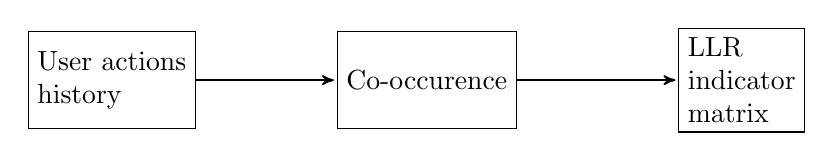
\begin{tikzpicture}[node distance=40mm,
data/.style={
rectangle,
draw,
thin,
minimum height=3.5em
},
to/.style={->,>=stealth',shorten >=1pt,semithick,font=\footnotesize},
]
\node (hist) [data, align=left] {User actions\\history};
\node (co) [data,right of=hist,align=left] {Co-occurence};
\node (in) [data,right of=co,align=left] {LLR\\indicator\\matrix};
\draw[to] (hist) -- (co);
\draw[to] (co) -- (in);
\end{tikzpicture}
\caption{To compute the indicator matrix we first count the co-occurrences of items and then we compute the log-likelihood strengths of the \glspl{coocc}.}
\label{fig:llrworkflow}
\end{figure}

\subsubsection{Log-likelihood ratio}
\label{sec:llrs}

\Gls{llr} is a probabilistic measure of the importance of a \gls{coocc}. The \gls{llr} similarity  is the probability that two users share the same items because the items are similar and not due to chance. It finds important \glspl{coocc} and filters out the coincidental. Hence it avoids that the result is skewed against popular items \cite{Dunning93}. Compared to the Jaccard coefficient \cite{Hartung} the log-likelihood-based similarity computes higher similarities for anomalous co-occurrences than for items that occur in every user history. For a detailed explanation of the math involved see \cite{Dunning93}. 

According to \cite{Dunning14} using the \gls{llr} ratio of the \gls{coocc} has several advantages.
\begin{itemize}
\item It yields good results for data that only captures the interaction and no explicit numerical \glspl{preference} value \cite{Dunning93}.
\item The similarity is not skewed against popular items.
\item We can use distributed MapReduce based algorithms to compute the \glspl{coocc}. Hence the computation of the \gls{llr} similarity is \gls{scalable}.
\end{itemize}

\subsubsection{Example}
\label{sec:llrexample}

We describe the log-likelihood based similarity with a small example data set. Suppose we analyze the user action history for the action ``like'' given in table \ref{tbl:llr1}. 
Table \ref{tbl:llr1} shows the likes of four users for five items. The items are represented with integers 1-4 and the users with integers 101 - 104  (see appendix listing \ref{lst:sampledata} for raw web log).
In the example data set of table \ref{tbl:llr1} the items 1 and 2 are similar because three users liked both of them.

We compute the \gls{indicatorm} in two steps as shown in figure \ref{fig:llrworkflow}.
\begin{enumerate}
\item Count \glspl{coocc}
\item Compute \gls{llr} of \glspl{coocc}
\end{enumerate}

\begin{table}
\begin{center}
\begin{tabular}{rllll}
 & 101 & 102 & 103 & 104\\
1 & x & x & x &  \\
2 & x &   & x & x\\
3 & x & x & x &  \\
4 &   & x & x & x\\
5 & x & x & x & x\\
\end{tabular}
\end{center}
\caption{Example data set. The columns represent the user interaction with an item. Items are named 1 - 4 and users 101 - 104}
\label{tbl:llr1}
\end{table}

In order to get the similarities between all items we count the \gls{coocc} of ``\glspl{like}'' for all item pairs. This leads to the $5 \times 5$ \gls{indicatorm} $C$ shown in equation \ref{eq:coocm}. The rows and the columns are items. $C$ is a similarity comparison of every row of table \ref{tbl:llr1} to every other row.

\begin{equation}
  \label{eq:coocm}
C =\bordermatrix{~ & 1 & 2 & 3 & 4 & 5 \cr
1 & 4 & 2 & 3 & 2 & 3 \cr
2 & 2 & 3 & 2 & 1 & 3 \cr
3 & 3 & 2 & 3 & 2 & 3 \cr
4 & 2 & 1 & 2 & 3 & 3 \cr
5 & 3 & 3 & 3 & 3 & 4 \cr}
\end{equation}

In the next step we compute the \gls{llr} ratio strength of the \glspl{coocc} for every item pair. This will again produce a $5 \times 5$ \gls{indicatorm}. Equation \ref{eq:coocm1} shows the \gls{indicatorm} for the sample data set from table \ref{tbl:llr1}.

\begin{equation}
  \label{eq:coocm1}
L =\bordermatrix{~ & 1 & 2 & 3 & 4 & 5 \cr
1 &   & 0.40 & 0.81 & 0.63 & 0 \cr
2 & 0.40 &  & 0.40 & 0.63 & 0 \cr
3 & 0.81 & 0.40 &  & 0.63 & 0 \cr
4 & 0.63 & 0.63 & 0.63 &  & 0 \cr
5 & 0 & 0 & 0 & 0 & \cr
}
\end{equation}

Although item 5 shares all users with item 1 and 3, the log-likelihood ratio is 0 because every user purchased item 5. The goal of collaborative filtering is to show the user items he would not find by himself. Item 5 is popular and a user will probably discover it by looking up a list of items sorted by popularity (this is a form of non-personalized recommendation). Hence Item 5 is not a valuable personal recommendation because we could extract it without a recommender. For this reason the \gls{llr} is suitable similarity metric for a recommender engine.

\subsubsection{Log-likelihood similarity implementation}
\label{sec:llrimpl}

Apache Mahout provides an implementation of log-likelihood similarity with the class \verb|LogLikelihoodSimilarity|. Unfortunately the LogLikelihoodSimilarity is a non-distributed implementation. It would take too long to calculate the indicator matrix for a data set with over 10 million items and we would have difficulties to load all data into the memory. 

The computation of the \gls{coocc} of every item pair can be distributed and run in parallel by applying the MapReduce programming model as follows:
\begin{description}
\item[Map] Determine all \glspl{coocc} for one user's history and yield a pair of items for each \gls{coocc}
\item[Reduce] For each item collect all corresponding item pairs of the map phase and count all \glspl{coocc} and yield a vector with all items and the corresponding \gls{coocc}.
\end{description}

This task can run in parallel on different nodes on a cluster computer framework, such as Apache Spark. Hence the computation of the \gls{indicatorm} is \gls{scalable}.
In order to compute the \gls{llr} similarity distributed on a Spark cluster, Apache Mahout provides the \verb|spark-item-| \verb|similarity| job. 
\verb|spark-itemsimilarity| is a command line job and we can start it from the Mahout shell.
\begin{verbatim}
./mahout spark-itemsimilarity --input $infile --output $outfile
\end{verbatim}
The job connects to the Spark cluster instance defined by the environment variable \verb|MASTER| and computes the \gls{indicatorm} in parallel. With the \verb|spark-itemsimilarity| job the indicator matrix can be computed in $O(n)$ \cite{Schelter}. 
The input text file contains a row for every user-item interaction. They have to be in the following format:
\begin{verbatim}
userID, action, itemID
\end{verbatim}
The output will be a text file that represents the indicator matrix as sparse vectors for every item. For every item we get the similarities to all other items.
\begin{verbatim}
itemID1<tab>itemID2:similarityvalue<space>itemID3:simvalue...
\end{verbatim}

In our demo application we have written a Python script to fetch the data from the sqlite3 database and transform to the Spark input format.


\subsection{Using more than one type of behavior}
\label{sec:multimodal}

Most collaborative filtering algorithms use only explicit or implicit ratings to compute similarity.
But we can improve the performance of the recommender engine by using multiple types of user actions. In addition to likes we could use tag-associations to compute the similariy. In table \ref{tbl:llr} we count co-occurence of items in a user's like-action history. Instead of the action history we could use tags that are associated width items. We count the co-occurence of each items associated with a tag.

Suppose we compute a \gls{indicatorm} based on likes $M_l$ and one based on tag associations $M_t$. An $h_l$ is a user's history of ``likes'' and $h_t$ is the user's tag history. Then we can compute the recommendation vector (see equation \ref{eq:recommendation}) $r$ with

\begin{equation}
  \label{eq:multi}
  r = h_l M_l + h_t M_t
\end{equation}

In our demo web application we use ``likes'' and tags but virtually all user actions can be used to improve the recommendation.

\subsection{Why can we use a search engine to produce \gls{topn}?}
\label{sec:relation}

The \gls{rec} uses a search engine to produce a \gls{topn}. We can deploy a search engine in order to provide recommendations because there are similarities between the computation of the \gls{topnt} and the retrieval of a ranked search result set.
 This section explains why the deployment of a search engine is suitable for the top-N recommendation task.

\subsubsection{Ranked retrieval}
A search engine enables user to search a collection of documents for specified keywords in a query. A document contains several \glspl{field}. A \gls{field} contains a sequence of terms or meta data about the document. A user can search for documents that contain keywords only in specific fields. The search engine returns a sorted set of documents that match the query. The result set is sorted by relevancy. The top documents are the most relevant to the query. This process is called \gls{rankedretrieval}. The search engine does this by calculating a similarity score between each document and the query and then sorts the result by this score. The score indicates the strength of the match against the query. This is one of the main use cases where search engines shine compared to relational databases. There a row either matches a query or it does not. 

\subsubsection{Vector space model}
One way to calculate the similarity between a query $q$ and a document $d$ is to use the vector space model.
In the vector space model each document $d$ and the query $q$ are represented as vectors $\vec{v}(d)$ and $\vec{v}(q)$. The vector contains an element for each term. It maps every term $t$ of the collection to a tf-idf weight. tf-idf reflects how important a term is to a document in the collection (see \cite{Manning} for a detailed description). 
The similarity score between two items is equal to the dot product.
\begin{equation}
  \label{eq:score}
  \text{score}(d,q) = \vec{v}(d) \cdot \vec{v}(q)
\end{equation}
In order to create a ranked result set for a query $q$ the search engine computes $\text{score}(d,q)$ for all documents in the collection. We can form a matrix $C$ with the document vectors as rows. The process of scoring all document can be written as matrix vector multiplication of $C$ and $q$. 
\begin{equation}
  \label{eq:ser}
  r = C q
\end{equation}
$r$ maps every document to a relevancy score.
This is similar to the computation of the \gls{topn} $r_u = M h_u$  described in section \ref{sec:problem}. The search engine returns documents with fields who's vector representation $\vec{d}$ is similar to the query vector $\vec{q}$. The recommender returns items that are similar to the items in the user's action history $h_u$. If we can map items to documents and the user's action history to a query we can use an existing search engine for the top-N recommendation task. This is desirable because search engines like Apache Solr are optimized for ranked retrieval and they are able to process big data at scale. 

\subsubsection{How to map documents to items}
\label{sec:mapping}

\begin{lstlisting}[caption={Item meta data and similar items are stored in Solr.},label={lst:solrdoc}]
{
    id: 1,
    title: Toy Story,
    tags:Pixar animation fantasy,
    likeindicator: 1688 1834 3893 4366 6281 33162,
    tagindicator: 10 33 41 54 55 59 66 67 72 73 80
    _version_: 1505056335358591000
}
\end{lstlisting}

The result of the search should contain a list of items. Hence we index items instead of documents.

Instead of finding documents that contain the keywords of the query in a field we want to find items that are similar to the items in the user's action history. We will first discuss a simple approach. 

For item $i$ we store all items whose \gls{llr} ratio (described in section \ref{sec:llrs} to $i$ is above a defined threshold in a separate field. For every type of user action we create such a field. These fields are called \glspl{indicatorfield}. 

Figure \ref{lst:solrdoc} shows an example entry of a movie item formatted in JSON. The indicator fields \verb|likeindicator| and \verb|tagindicator| contain movie ID's of similar movies. In addition to the indicator fields, the entry contains meta data about the item. These fields can be used to retrieve items by meta data, such as title or genre.

We query the search engine with items from the user's action history $h$. The search engine will transform the items in the query to the corresponding document vector. Table \ref{tbl:comparison} shows the mapping.

This way the search engine computes a higher score for documents that contain the items in $h$ also in their indicator fields. The more items the query $h$ and an indicator field of $i$ have in common the higher the similarity score for a document. Hence the search engine returns similar items the user already liked. In addition the tf-idf weights of the document vectors will mitigate popular items. The drawback of this simplified approach is that it does not account for different \gls{llr} similiarity values betwenn items above threshold. They are ignored.

 We want to have some way to include the \gls{llr} ratios of the \gls{indicatorm} $M$ to boost items that have a high similarity to the item represented by the document. In order to include the similarity metric among items described in section \ref{sec:llr} we have to weight the tf-idf values in the document vector with the \gls{llr} ratios. This is the reason why we can't use a search engine out of the box without extending it's scoring function. 

\begin{table}
\begin{center}
\begin{tabular}{lll}
 search engine & \gls{rec}\\ \hline
  document & item\\ 
 field & indicatorfield \\
 term & item (item id)    \\
 query & user's action history \\
payload & LLR similarity \\
\end{tabular}
\end{center}
\caption{We can map document, fields, term and query to the recommender equivalents.}
\label{tbl:comparison}
\end{table}

\subsubsection{Emulate different recommender strategies}

Note that we can emulate different recommendation engines by using different queries.
\begin{itemize}
\item If the query is composed with the user's action history we use collaborative filtering with an \gls{itembased} approach.
\item We can use a single item $i$ as query and get back all similar items. For instance, a top-N list of items retrieved with this query can be placed on a description page of item $i$ with the title ``Customers Who Liked This Item Also Liked''. This is a non-personalized approach.
\item We can use user profile information in the query. If the user profile contains information about the user's favorite movie genre or favorite director and the search engine has indexed the corresponding meta data we can search for items that match the user' profile. This would be a content based approach.
\end{itemize}

\subsubsection{Implementation}
\label{sec:solrimpl}
We deploy the search engine Apache Solr in our demo webapplication. Simply put, Solr is a Web API for Apache Lucene, an open source information retrieval software library. 

In order to use the precomputed \gls{llr} ratios of the \glspl{coocc} we need a way to store them per term and per document. Lucene provides this functionality with the \emph{playloads} feature. Payloads enable an application to store an arbitrary byte array for every term during indexing \cite{McCandless}.

Unfortunatly the feature is only implemented in Lucence, not in Solr. But we can extend Solr to use the Java classes that deal with payloads.

First we need to define a new fieldtype in the schema.xml of our Solr configuration. Fields of this type contain terms with an added payload.
To index the similarity value we define a custom fieltype that uses Lucene's DelimitedPayloadTokenFilter to extract a payload from every term. 

\begin{lstlisting}[caption={Fieldtype definition for field with payload.}]
<fieldtype name="payloads" class="solr.TextField" >
 <analyzer>
  <tokenizer class="solr.WhitespaceTokenizerFactory"/>
   <filter class="DelimitedPayloadTokenFilterFactory" />
 </analyzer>
</fieldtype>
\end{lstlisting}
The default delimiter is the pipe symbol. With this fieldtype we can add payloads to terms in document be attaching a number to the term string.
\begin{verbatim}
23|0.9
\end{verbatim}
In this example \verb|23| is an item-id and \verb|0.9| is the similiarity value to the corresponding item.

After we stored the payload within the index we need a way to score a document match according the payload.
Solr uses per default the vector space model to compute the score between a document $d$ and a query $q$. It only considers terms $t$ that appear in the query $q$. The tf-idf weight is multiplied by a boosting factor for a term $t$ \cite{grainger}.  
\begin{equation}
\label{eq:solrsim}
\text{score}(q,d) = \sum_{t \in q} \text{tf-idf}(t,d) \cdot \text{boost}(t)
\end{equation}

In order to use the payload values in the ranked retrieval process we have to extend Solr with our own Query Component. 

We can add a custom Query Component by implementing a \verb|QParserPlugin|. The implementation just returns the \verb|PayloadTermQuery|. \verb|PayloadTermQuery| matches all documents containing the specifed term and than applies a scoring factor based on the payload that is stored with each term.

In addition we have to override the method \verb|scorePayload| of the \\ \verb|DefaultSimilarity| class. \verb|PayloadTermQuery| will call \verb|scorePayload| to determine the payload of an item and then it multiplies the td-idf weights with the corresponding payload. We have to tell Solr to use our custom Query Component and the new \verb|PayloadSimilarity| by adding the following entries to the solrconfig.xml.

\begin{lstlisting}
<similarity class="ch.hsr.solrpayload.PayloadSimilarityFactory">
<queryParser name="payloadparser" 
   class="ch.hsr.solrpayload.PayloadParser" />
\end{lstlisting}
  
Solr will load the implementations from it's \verb|lib| directory if we package them Java jar archive.

\begin{figure}
  \centering
\begin{tikzpicture}
  \begin{axis}[
    title=evaluation of LLR threshold,
    xlabel=threshold,
    ylabel=Precision/Recall,
    width=10cm,
    ]
\addplot table {thresholdp.dat};
\addplot table {thresholdr.dat};

  \end{axis}
\end{tikzpicture}
\caption{The precision and recall at 10 for the MovieLens data set is measured as a function of the similarity threshold. Items with a small similarity value do not contribute to the performance. The best performance is archieved by only adding items with a \gls{llr} ratio above 0.9.}
\label{fig:threshold}
\end{figure}

In our demo web application we only add items above a given \gls{llr} ratio threshold to the index of the search engine. If we add items with a small similarity to the indicator fields the precision and recall decline. The evaluation in figure \ref{fig:threshold}shows that the we archieve the best performance with a threshold of 0.9.

An alternative to the use of payloads is to ignore similarities values once we removed the item below threshold from the index. In that case the scoring of a document only depends on the tf-idf weight. Only add items above a threshold to the indicator fields. This approach is easier to deploy but it doesn't account for different similaries. 

\section{Integration}
\label{sec:integration}

This section will describe the integration of the \gls{rec}. In section will describe how we integrate components described in section \ref{sec:design.}

The recommender discussed in this report has to parts.
\begin{description}
\item[Compute similarities] In this part the user action are analised in order to compute the similarities of items. The similiarities are stored as indicators in Apache Solr.
\item[Generate personalized recommendations] A systems formats a list of recommended items.
\end{description}


\subsubsection{Retrieve recommendation}

In order to produce recommendations we compose a Solr query from the user history. The user history is stored in the web log. The web server sends this query to Solr. Solr responds with a ranked result set. The web server then formats the response from Solr and sends a list of recommended items to the user.

\begin{figure}
\centering
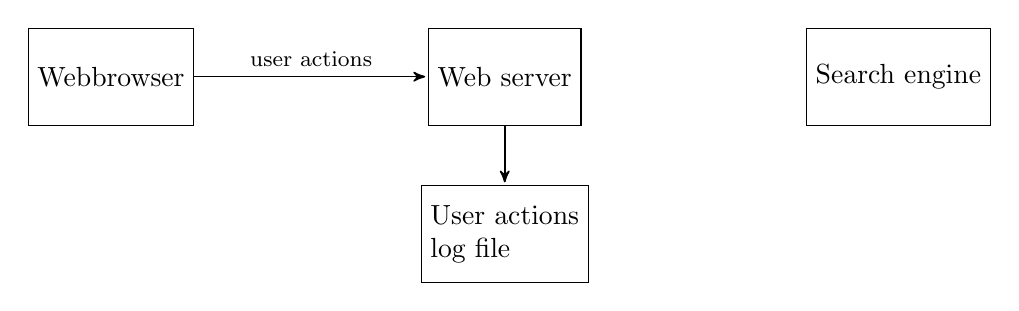
\begin{tikzpicture}[node distance=20mm,
data/.style={
rectangle,
draw,
thin,
minimum height=3.5em
},
to/.style={->,>=stealth',shorten >=1pt,semithick,font=\footnotesize},]

\node (web) [data] {Web server};
\node (log) [data,below of = web, align=left] {User actions\\log file};
\node (browser) [data,left of=web,node distance=50mm] {Webbrowser};
\node (solr) [data,right of=web,node distance=50mm] {Search engine};
\draw[to] (web) -- (log);
\draw[to] (browser) -- node[midway,above] {user actions} (web);
\end{tikzpicture}
\caption{The web server sends this query to Solr. Solr responds with a ranked result set.}
\end{figure}

\verb|updatesearchengine| will index all movies in Solr.

Solr is used in the offline and the online part of the recommendation engine.

The items and their corresponding similarity indicators from the Apache Spark job are stored with Apache Solr. 

We store all items as documents in Solr. The documents contain the metadata like (title, genre, tags, etc). In addidtion we populate a filed for every indicator with the similar item ID's discovered with the coocuccence similartiy from section \ref{sec:llr}.

In order to build a recommender using a search engine we store the output of the co-occurence analysis in Solr. The search engine actually delivers the recommendations to our users.

\subsection{Parameters}
\label{sec:parameters}

This section descripes the paratemter of the recommender discussed in this report.
\begin{description}
\item[similarity threshold] We have to define a threshold to separate similar items occording to the LLR similarity from the rest (e.g. 0.5).
\item[user history to consider] We retrieve recommendations with a part of the user history. We have to define the number of log entries to consider.
\end{description}

\subsection{Two-parts design}

The recommender described in this article is divided in two parts.
\begin{itemize}
\item Computation of simililarity and the update of the text search engine is done offline, ahead of time.
\item Recommendations are generated instantly by quering the text search engine using rescents actions of the user.
\end{itemize}

\section{Evaluation}
\label{sec:evaluation}

This section describes the evaluation process and presents the results of the evaluation. In order to run the evaluation we created a small Java project called \verb|evaluator|. It contains the classes to evaluate the performance of the recommender discussed in this report and the Top Popular recommender (see section \ref{sec:baseline}). We use the MovieLens data set as training and test data set. Note that this data set contains preference values.

Evaluation is important because:
\begin{itemize}
  \item It allows us to decide if the quality of the recommender engine archives the desired results. 
  \item We are able to compare the discussed approach to other recommender algorithms. It allows us to compare different recommender techniques.
  \item Evaluation allows us to adjust the parameters in order to get better results.
\end{itemize}

\subsection{How to measure the performance of the \gls{topnt}?}

Most commonly accepted evaluation measure for recommender systems is the Mean Average Error or Root \gls{mae} of the predicted ratings and the actual one \cite{Ricci}\cite{jannach11}.
As decribed in section \ref{sec:problem} the \gls{rec} does not estimate preference values. It produces a \glspl{topn}. Hence we can not use \gls{mae} as a performance metric. 

We can look at the recommender problem as a classification problem. The recommender engine assigns every item into the category of recommendable items or unimported items.
If we look at the recommender problem as a classification problem we can make use of precision and recall to evaluate the performance. Precision and \gls{recall} are two \gls{ir} concepts \cite{Manning}. We provide a brief summary here to each of these measures.

Precision and recall depend on the following measures.
\begin{description}
\item[True positive (TP)] Number of items classified as recommendable or relevant that are truly of interest to the user. 
\item[True negatives (TN)] Number of instances not contained in the recommendation list (classified as irrelevant) and that in fact are not of interest to the user.
\item[False positives (FP)] Number of instances recommended but are not relevant to the user.
\item[False negatives (FN)] Number of instances not shown in the recommendation list but that in fact are relevant to the user.
\end{description}


\begin{figure}
\centering
\begin{tikzpicture}[
box/.style={draw,rectangle,minimum size=3cm,text width=2.5cm,align=left}]
\matrix (conmat) [row sep=.1cm,column sep=.1cm] {
\node (tpos) [box,
    label=left:Relevant items,
    label=above:,
    ] {relevant \\ recommendations \\ (TP)};
&
\node (fneg) [box,
    label=above:,
    label=above right:,
    label=right:] {relevant\\ but not \\recommended\\(FN)};
\\
\node (fpos) [box,
    label=left:irrelevant items,
    label=below left:,
    label=below:Top-N list] {irrelevant \\but\\recommended};
&
\node (tneg) [box,
    label=right:,
    label=below:not in Top-N list] {irrelevant\\and not\\recommended};
\\
};
\node [left=.05cm of conmat,text width=1.5cm,align=right] {\textbf{actual \\ prefences}};
\node [above=.05cm of conmat] {\textbf{recommender classification}};
\end{tikzpicture}
\caption{Confusion matrix for top-N recommendation task}
\label{fig:confusionmatrix}
\end{figure}

Figure \ref{fig:confusionmatrix} visualizes the measures used for precision and recall. This table is called confusion matrix or contingency table \cite{Manning}. 

\subsubsection{Precision and Recall}
\label{sec:precision}

\begin{description}
\item[Precision] Precision is the proportion of items in the top-N list of recommendatoins that are relevant \cite{Manning}.
  \begin{equation}
    \label{eq:precision}
    \text{Precision} = \frac{\text{number relevant items recommended}}{\text{size of the recommendation list}}
  \end{equation}
We can formulate this with the measures from the confusion matrix.
  \begin{equation}
    \label{eq:precisionm}
    \text{Precision} = TP/(TP+FP)
  \end{equation}

 Suppose the recommender create a list of 5 items. If 3 items are relevant recommendations then the precision is $3/5$. 
Precsion only considers the accuracy of the recommendation list and not the comprehensiveness of the result.

\item[Recall] Recall is the proportion of relevant items that appear in the recommendation result. 
  \begin{equation}
    \label{eq:recall}
    \text{Recall} = \frac{\text{number relevant items recommended}}{\text{relevant items}}
  \end{equation}
  \begin{equation}
    \label{eq:recallcm}
    \text{Recall} = TP/(TP+FN)
  \end{equation}
Suppose there are 9 relevant recommendations. If the recommender results contains 3 of these relevant recommendations then the recall is 3/9.

Note that recall should not used without precision. We could build a recommender with perfect recall by recommending all items.
\end{description}

\subsubsection{Implementation}
\label{sec:irimpl}

Listing \ref{lst:irstats} shows the implementation of precision and recall. 
The variable \verb|rec| contains an object of type \verb|Recommender|. \verb|Recommender| provides the method \verb|recommend|. \verb|recommend| takes the ID of the active user and the size $N$ of the top-N list as parameters. The argument \verb|topNsize| corresponds to $TP+FP$. It returns a top-N list for the active user. 

The variable \verb|relevantItemIDs| contains a list with relevant items for the active user.

We count how many items in the top-N list are also in the list \verb|relevantItems| and assign the result in \verb|relevantItemsRetrieved|. \verb|relevantItemsRetrieved| corresponds to the $TP$ value. In order or compute precision or recall we divide \verb|relevantItemsRetrieved| by \verb|topNsize| or the size of the collection\\ \verb|relevantItems|.


\begin{lstlisting}[caption=Implementation of precision and recall,label=lst:irstats]
double precision = 0;
double recall = 0;
int relevantItemsRetrieved = 0;

List<RecommendedItem> recItems = rec.recommend(userID, topNsize);
   for (RecommendedItem recItem : recItems) {
	if (relevantItem.contains(recItem.getItemID())){
			relevantItemsRetrieved++;
	}
   }

// Precision
int numRecommendedItems = reItems.size();
precision = ((double) relevantItemsRetrieved / (double) topNsize);
		      
// Recall
recall =  relevantItemsRetrieved / (double) relevantItems.size());
		      
\end{lstlisting}

\subsection{Testing Methodology}
\label{sec:methodology}
The definitions \ref{eq:precision} and \ref{eq:recall} of precision in recall rely on the number of relevant items.
If we want to evaluate a recommender with \gls{precision} and \gls{recall}, we have to define, what is a relevant item for the active user. 

Relevancy depends on the goal of the recommender. For example, an item is relevant if the user would give it a high rating or if he would purchase the item but he is not aware of it.
Those items are unknown at the time of the recommendation. 

Unfortunatly we do not know if a user likes some new item in the future.
But we can simulate the prefencences of the future by setting aside a small part of the real data set as test data.

In order to separate the test data set from the training data set we get all ratings of user $u$. We sort these rating according the rating value. Then we select the top $N$ items $T$ that are greater then a given threshhold $t$ from the sorted list. Items in $T$ have a high rating and we assume they are relevant to the user $u$. Items in $T$ form the set $TP + FN$ (see figure \ref{fig:confusionmatrix}). 
The threshhold prevents us from adding items with a low rating to $T$. If a user rates three items with the rating 5.0, 1.0 and 1.0 the evaluation algorithm would add the items with the bad rating 1.0 to $T$. Hence the items with bad rating 1.0 lead to lower recall measures. 
If there are no numerical rating values but only Boolean values we have to select $N$ items at random.

All ratings in $T$ are removed from the overall input set. The remaining preferences form the training data set $M$. In order to measure precision and recall we first train the recommender with the data in $M$. For instance, if we evaluate a co-occurence based recommender we compute indicator matrix from section \ref{sec:llr} with this set.

We use the trained recommender to form the \gls{topn} for user $u$. This list corresponds to the set $TP + FP$ in the confusionmatrix.

We check how many items are contained in the top-N list that are in $T$. These items are the set $TP$ (see figure \ref{fig:confusionmatrix}). 

For example, if $N$ is 5 this would mean \gls{precision} and \gls{recall} are evaluated by removing the top 5 preferences for a user and then finding the percentage of those 5 items included in the top-N recommendation list for that user. 

In short the evaluatuation process for a single user $u$ can be devided into several steps:
\begin{enumerate}
\item Retrieve relevant items $T$ for user $u$ ($TP+FN$).
\item Build the training set $M$ by removing the corresponding preferences from input data set.
\item Train the recommender engine with $M$.
\item Form a \gls{topn} for $u$ ($TP+FP$).
\item Count the number of items that appear in the top-N list and in $T$ ($TP$).
\item Compute precision and recall based on $TP$, $FP$ and $FN$.
\end{enumerate}

The evaluation process has the following parameters:
\begin{description}
\item[Size of the result] The length $N$ of recommendations list and number of the relevant items. 
\item[Relevance threshold] Determines if an item is relevant or not.
\end{description}

\subsection{Baseline algorithms}
\label{sec:baseline}

In order to get a feel what values of precision an recall to excpect and to determine the performance of the search engine based, multimodal recommender we compare it with three base line algorithms. 

\begin{description}
\item[Random] The recommender randomly recommends $N$ items to the user. This algorithms serves just as baseline for the more complex algorithms.
\item[Top popular]  It creates a list of items ordered by the numbers of ratings for a specific item. Top Popular is a non-personalized recommender because it presents the same list of items to any user \cite{Cremonesi}. Listing \ref{lst:toppop} shows the implementation of the the Top Popular algorithm. 

\begin{lstlisting}[label=lst:toppop, caption={Implementation of top popular recommender}]
Map<Long, Integer> item2pop = new HashMap<Long, Integer>();
LongPrimitiveIterator iter = dataModel.getUserIDs();
while (iter.hasNext()) {
PreferenceArray prefs = dataModel.getPreferencesFromUser(iter
	.nextLong());
for (int i = 0; i < prefs.length(); i++) {
	Integer counter = item2pop.get(prefs.getItemID(i));
	if (counter == null) {
		item2pop.put(prefs.getItemID(i), 1);
	} else {
		item2pop.put(prefs.getItemID(i), counter + 1);
	}
      }
}
List<RecommendedItem> popitems = transfom2list(item2pop);
Collections.sort(itemidcounter, new RecommenderItemComparator()); 
return popitems
\end{lstlisting}

\item[Item-based with cosine similarity]  \Gls{itembased} collaborativ filtering is a model-based, collaborative filtering algorithm. It computes the simililarities between all items and predicts user prefences by based one existing ratings. We use the cosine similarity \cite{ekstrand11} to measure the similarity between two items. The \gls{itembased} algorithm selects $k$ neirest neighbors $N$ of $i$. It then weights the ratings of the active user $u$ for each item $i'$ in $N$ with the similarity $sim(i,i')$ and compute the sum of that. The predicted rating $r_{u,i}$ for user $u$ and item $i$ is the normalized value of the sum \cite{jannach11}:

\end{description}
\begin{equation}
  \label{eq:computeprediction}
  r_{u,i} = \frac{\sum_{i' \in N}{sim(i,i') r_{u,i}}}{\sum_{i' \in N}{|s(i,i')|}}
\end{equation}

We use Mahouts implementation of an \gls{itembased} recommender. Mahout provides the \verb|GenericItemBasedRecommender| class with an implementation of an \gls{itembased} recommender. To compute the similiarty we use \verb|UncenteredCosineSimilarity|.

\subsection{Dataset}
\label{sec:dataset}

The testing methodology of section \ref{sec:methodology} requires an existing data set. We used ratings and tagging activity from MovieLens, a movie recommendation service \cite{movielensdata}.
MovieLens data sets were collected by the GroupLens Research Project at the University of Minnesota. The data was collected through the MovieLens web site (movielens.umn.edu) during the seven-month period from September 19th, 1997 through April 22nd, 1998 \cite{movielensdata}.

This data set consists of:
\begin{itemize}
\item 100,000 ratings. The ratings are scores from 1 to 5. A rating is made by one user to one movie at a specific time. 

\item 943 users. Each user has rated at least 20 movies
\item 1682 movies. Movies are categorized in genres. A movie has an ID, a title, and a list of associated genres. 
\item 2488 \gls{tag} appliciations. A \gls{tag} is applied by one user to one movie at a specific time. Tags are user-generated metadata about movies. Each tag is typically a single word or short phrase. The meaning, value, and purpose of a particular tag is determined by each user.
\end{itemize}
 
We choose this dataset due to several reasons:
\begin{itemize}
\item It contains ratings and tagging activity. Hence we can use two indicators for the multimodal co-occurence based recommender.
\item As described in section \ref{sec:methodology} we need numerical rating scores to select the top $N$ ratings of a user in order to form a test set. 
\item  It is common to evaluate a recommender engine with it. Hence it is easier to compare the results with other recommender engines. 
\end{itemize}

The co-occurence based recommender takes user actions as Boolean values as an input. The MovieLens data set contains preferences with a numerical rating score. 
In order to simulate the user action ``like'' as described in section \ref{sec:inputdata} we generate a new data set based on the MovieLens data set. We select all preferences with a score equal or above 4.0. These \glspl{preference} indicate that the user likes the item hence we consider them as likes.

\subsection{Evaluationresults}
\label{sec:results}
To compare the \gls{rec} with the baseline algorithms (described in section \ref{sec:baseline}) we use three \glspl{indicator}.

\begin{description}
\item[Co-occurence user likes] As described in section \ref{sec:dataset} we generate a user action history with ``like'' actions. We calculate the \gls{llr} strengths between all items and use the rrecent likes in the user's history as query.
\item[User ratings] We use the \gls{coocc} based similiarity metric descibed in section \ref{sec:}the preference values to calculate the  similarity between all items.
\item[Tags] We use the tags associated with an item to compute a tag \gls{indicator} matrix. We use the tags associated with the user to create a query.
\end{description}

We created three recommenders. We measure precision and recall first with the recommender ``1.indicator'' that only considers co-occurence of user likes. Then we add the indicator ``user ratings'' to the multimodal recommender ``2 indicators'' and then we use all 3 indicators to retieve a \gls{topn} (``3. indicators''). 

We measure precision and recall at $N=10$. Hence we retrieve a list of 10 items. Relevant items are the 5 best rated items above a threshold of $\mu + \sigma$ all user ratings.

\pgfplotsset{width=7cm}
\begin{figure}
  \centering
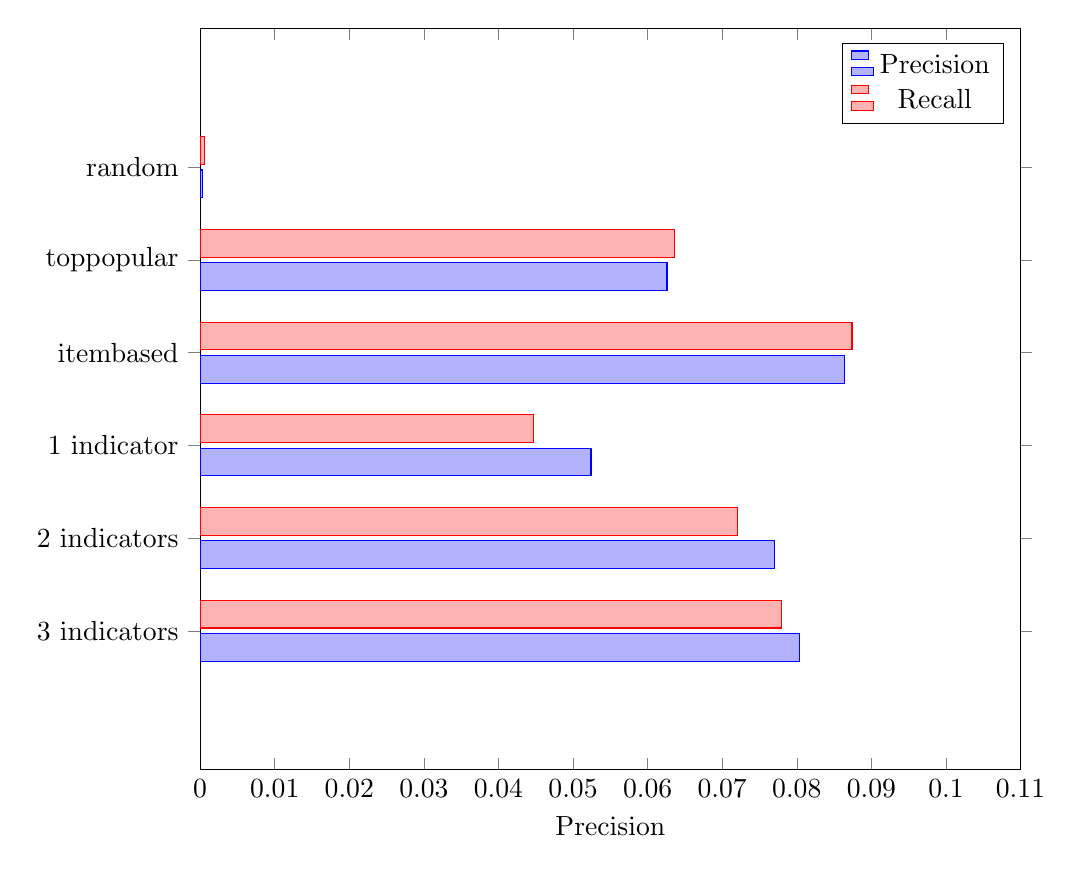
\begin{tikzpicture}
\begin{axis}[
xbar,
xmin=0,
xmax=0.11,
width=12cm,
height=11cm,
enlarge y limits=0.3,
xlabel={Precision},
symbolic y coords={3 indicators,2 indicators,1 indicator,itembased,toppopular,random},
ytick=data,
x tick label style={/pgf/number format/fixed}
]

\addplot coordinates {(0.00035,random) (0.0626,toppopular) (0.0864,itembased) (0.0524,1 indicator) (0.077,2 indicators) (0.0804,3 indicators)};
\addplot coordinates {(0.00054,random) (0.0636,toppopular) (0.0874,itembased) (0.0447,1 indicator) (0.072,2 indicators) (0.078,3 indicators)};
\legend{Precision, Recall};
\end{axis}
\end{tikzpicture} 
\caption{Precision comparison of recommender algorithsm, random generated recommendations, Top Popular and itembased with precision at 10 and $N$ = 10 (number of recommended items)}
  \label{fig:precisionrecallvalues}
\end{figure}

Figure \ref{fig:precisionrecallvalues} shows the comparison of \gls{coocc} based recommender with one, two and three indicators with the baseline algorithms from section \ref{sec:baseline}.
The multimodal co-coccurence  achieves an average precision and recall of 8 and 7.8 percent. This seems low. The recommender rarely recommends an item that the user liked explicitly. On the other hand we do not know if the recommended items are appealing to the user if he never rated them.

The evaluation shows that the quality of the recommender increases when we take more indicators into account. If we use just the user action ``like'' precision and recall are 5.2 and 4.5 percent. If we use user ratings and tags as indicator precision and recall are  8 and 7.8 percent. That an increase of 53 and 73 percent.

Compared to the baseline algorithms the \gls{coocc} based recommender achieves the second best results. It performs better than the non-personalized TopPopular algorithm and slightly worse than the itembased algorithm. The reason for this is the lack of a relevancy score for the similarities. The itembased algorithms considers the similirity value. The search engine does not have this information. Either a item id is part of a indicator field or not. This circumstance could be improved by using payloads in Solr. Another interesting fact is that the non-personalized algorithm almost match the quality of the more sophisticated approaches. Compared to randomly generated recommendations the \gls{coocc} improves the quality with a factor of about 250.

\section{Conclusion}
\label{sec:similarity}

A large amount of work was required to convert formats between the user logs the Apache Mahout and Apache Solr.

The system may be improved throug 
\begin{description}
\item[Dithering] 
\item[Anti-flood] 
\item[Cross-coooccurence]
\end{description}
dithering.

Mahout provides a large set of recommender algorithms. And it is easy to evaluate and compare several algorithms on a specific dataset.

\section{Infrastructur}
\label{sec:infrastructur}

\subsection{Webapplication}
\label{sec:web}

To start the Webapplication run:
\begin{verbatim}
sbt build 
\end{verbatim}


\appendix

\subsection{Apache Spark}
\label{sec:spark}
\verb|spark-rowsimilarity| is a script that comes with spark. It takes as input a text file representation of a matrix of sparse vectors. It finds similar rows. The input is in text-delimited form where there are three delimiters used. By default it reads (rowID<tab>columnID1:strength1<space>columnID2:strength2...) The job only supports LLR similarity. This job only supports LLR similarity.
The input has the following format:
\begin{verbatim}
1	1
2	2
3	3 
\end{verbatim}


\tikzset{
 mynode/.style={rectangle,rounded corners,draw=black, top color=white, bottom color=yellow!50,very thick, inner sep=1em, minimum size=3em, text centered}
}
\tikzstyle{format} = [draw, thin, fill=blue!20]
\tikzstyle{medium} = [ellipse, draw, thin, fill=green!20, minimum height=2.5em]
\begin{figure}
\centering
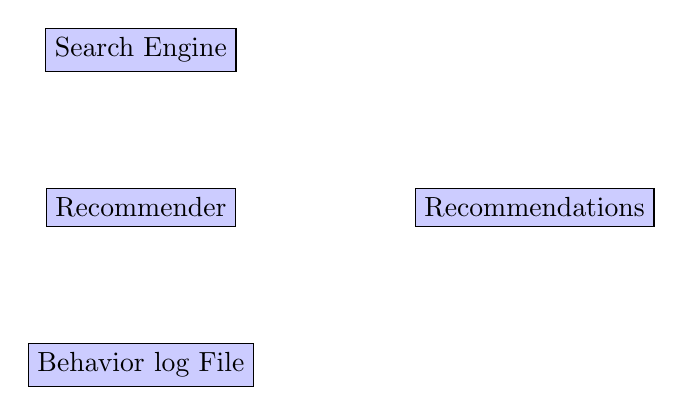
\begin{tikzpicture}[node distance=20mm,
data/.style={
rectangle,
draw,
thin,
fill=blue!20
}]
\node (recommender) [data] {Recommender};
\node (topn) [data,right of = recommender, node distance=50mm] {Recommendations};
\node (history) [data,below of = recommender] {Behavior log File};
\node (db) [data,above of= recommender] {Search Engine};
\end{tikzpicture}
\caption{Recommender engine}
\end{figure}

\section{Sample Input Data}
\label{sec:sampleinput}

\begin{verbatim}
itemid, userid, timestamp
1,101,980730861
1,102,980731380
1,103,980731926
2,101,980732037
2,103,980730408
2,104,980731766
3,101,980731282
3,102,980730769
3,103,980731208
4,102,980732235
4,103,980731417
5,101,980731745
5,102,980731621
5,103,980731417
5,104,980731208
\end{verbatim}


\section{Case Study: artoffer.ch}
\label{sec:artoffer}

The following action are used as indicators
\begin{itemize}
\item When a user visits the page of a item. (boolean)
\item When a user likes an item.
\item Tags
\end{itemize}
\bibliographystyle{plain}
\bibliography{a}
\end{document}
